\documentclass[sigconf, screen=true, anonymous=true]{acmart}

\usepackage{booktabs}
\usepackage[ruled]{algorithm2e} % For algorithms

\usepackage{siunitx}
\usepackage{graphicx}
\usepackage{multirow}
\usepackage[capitalise]{cleveref}

% For editing
\usepackage{ulem}
\usepackage{todonotes}

\renewcommand{\algorithmcfname}{ALGORITHM}
\SetAlFnt{\small}
\SetAlCapFnt{\small}
\SetAlCapNameFnt{\small}
\SetAlCapHSkip{0pt}
\IncMargin{-\parindent}

% Metadata Information
\acmConference{SAP}{September 2019}{Barcelona}
%\acmVolume{9}
%\acmNumber{4}
%\acmArticle{39}
%\acmYear{2010}
%\acmMonth{3}
%\acmArticleSeq{11}

%Copyright
\setcopyright{usgovmixed}

% DOI
\acmDOI{0000001.0000001}

% Paper history
\received{May 2019}

\begin{document}

\title{Audio Interface of an Active Perception Navigation Aid for People with Visual Impairments}

\author{Jacobus C. Lock}
\affiliation{%
  \institution{University of Lincoln}
  \streetaddress{Brayford Pool}
  \city{Lincoln}
  \state{Lincolnshire}
  \postcode{LN6 7TS}
  \country{United Kingdom}}

\author{Iain Gilchrist}
\affiliation{%
  \institution{University of Bristol}
  \streetaddress{Priory Road}
  \city{Bristol}
  \state{Bristol}
  \postcode{BS8 1TU}
  \country{United Kingdom}}

\author{Grzegorz Cielniak}
\affiliation{%
  \institution{University of Lincoln}
  \streetaddress{Brayford Pool}
  \city{Lincoln}
  \state{Lincolnshire}
  \postcode{LN6 7TS}
  \country{United Kingdom}}

\author{Nicola Bellotto}
\affiliation{%
  \institution{University of Lincoln}
  \streetaddress{Brayford Pool}
  \city{Lincoln}
  \state{Lincolnshire}
  \postcode{LN6 7TS}
  \country{United Kingdom}}

\begin{abstract}
	Our aim is to build a portable active navigation system for the visually impaired that uses active perception techniques and a combination of feedback modes to identify a scene and guide a user to their destination.
	Such a system requires a non-visual feedback interface and in this paper we investigate the effectiveness of a spatial audio tone with a varying pitch component, played through bone-conducting headphones, in conveying the pan and tilt angles of a target to the user in a pointing task.
	The goal is to determine how changes to the rate of change of the pitch affects a user's performance.
	For this, we conducted a set of experiments with blindfolded and visually impaired users and found that the varying pitch component gives an average error of approximately \SI{20}{\degree} when searching for a target; in line with previous results from other authors.
\end{abstract}

 \begin{CCSXML}
<ccs2012>
<concept>
<concept_id>10003120.10003121.10011748</concept_id>
<concept_desc>Human-centered computing~Empirical studies in HCI</concept_desc>
<concept_significance>500</concept_significance>
</concept>
<concept>
<concept_id>10003120.10003121.10003122.10003334</concept_id>
<concept_desc>Human-centered computing~User studies</concept_desc>
<concept_significance>300</concept_significance>
</concept>
</ccs2012>
\end{CCSXML}

\ccsdesc[500]{Human-centered computing~Empirical studies in HCI}
\ccsdesc[300]{Human-centered computing~User studies}

\keywords{Human-machine interface, vision impairment, spatialised sound, varying pitch, pointing task}

\maketitle
\renewcommand{\shortauthors}{JC Lock et al.}

\section{Introduction}

In recent years, governments have spearheaded numerous initiatives to support people with disabilities and enable them to play a more active role in modern society.
In the UK, the Royal National Institute of Blind People (RNIB) has prioritised enabling people with visual impairments to use some of the services and products many people take for granted, such as public transport and cellphones~\cite{rnib-objectives}.
Improvements in modern computing have made it possible for new and innovative solutions for these problems to come to the fore.
In particular, researchers in the active vision field have have made much progress in enabling machines to autonomously manipulate cameras to gather information about an environment for mapping and object and face tracking tasks~\cite{bajcsy2018revisiting}.
There is, however, a significant research question about whether techniques from active machine vision can be applied to humans, i.e.\ can a machine identify a point of interest in a scene and direct a human, instead of an electronic servo, to focus on that point?
If this can be done, it would be beneficial to people with visual impairments and will augment their ability to search for an arbitrary point or object of interest and identify an unknown scene. 

To this end, we are developing a mobile navigation system using a Google Project Tango tablet device\footnote{https://developers.google.com/tango}, pictured in \cref{fig:tango-headphone}, that caters to the perception limitations of people with limited vision by using a non-visual interface.
This system will ultimately allow users with visual impairments to reach a target location in the final leg of their journey, i.e.\ the so-called `last 10 yards' problem~\cite{google2016blind,bellotto2013}. 
The ideas here can also be extended and applied to mainstream navigation tools, such as Google Maps.
A Tango-enabled device comes pre-equipped with powerful image-processing, localisation and depth-perception capabilities and is built on top of a standard Android platform, providing access to the entire set of input/output options that this operating system has to offer.
%The final system will use multiple feedback modes (vibration, audio and voice) to guide a user toward a target destination while providing information on any oncoming obstacles.

\begin{figure}
  \centering
  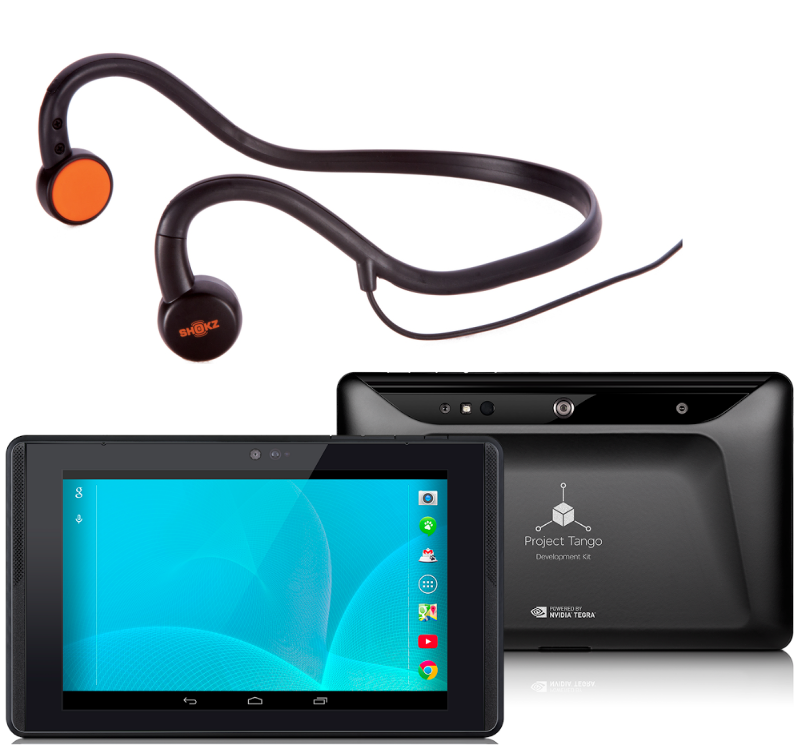
\includegraphics[width=0.5\columnwidth]{figures/tango_headphone.png}
  \caption{The Tango device and bone-conducting headset the system is based on. }\label{fig:tango-headphone}
\end{figure}

For this work, we implemented and evaluate an audio guidance mode that will be implemented in the guidance system to provide navigation instructions to the user. 
To evaluate this guidance mode, we conducted a set of experiments involving a target-search task where the participants were guided to point a camera to a set of virtual targets with the audio instructions.
The system uses a set of bone-conducting headphones to provide the audio instructions, with the latter being used to avoid interfering with a user's normal hearing function; something people with limited vision typically rely upon. 
However, this type of headphones bypass the external structure of the ear which provide the ability to localise a sound source's elevation.
We therefore use a tone of varying pitch to convey the target's tilt position w.r.t.\ the camera's pointing vector, $C$, pictured in \cref{fig:cam-coords}.
The tone is spatialised to provide the target's position in the pan dimension.
A similar interface can be found in~\cite{durette2008visuo}, where they used a varying pitch component without spatialising the tone. 
However, they did not investigate this interface's target-finding accuracy.
Furthermore, we wish to determine how changing the pitch's rate of change will affect target-finding performance. 
Therefore, this work contributes by determining how accurately a spatialised tone with varying pitch can direct a user towards a target, and how the pitch's rate of change affects this accuracy.

%In this paper we focus on the audio feedback mode and discuss how it is used in our system.
%We present experiments we performed to determine its effectiveness at directing a user to complete a pointing task and how its parameters affect users' target-search performance.
%For the pointing task, we presented blindfolded and partially sighted participants with a set of virtual targets, one after another, and asked them to point a camera to where they thought the targets were.
%The targets' pan and tilt angles w.r.t.\ the device's vertical plane, shown in \cref{fig:cam-coords}, were given to the participants through a spatial tone with varying pitch played via a set of bone-conducting headphones.
%We use the latter to not interfere with the user's normal hearing function, which people with visual impairments typically rely on.
%Because these headphones bypass the external structure of the ear responsible for localising a sound source's elevation, it is necessary to convey the target's tilt angle using another method.
%Therefore, we opted for a tone with varying pitch to convey the angle adjustment required to point the camera in a particular direction.
%A similar audio interface was successfully implemented and evaluated in~\cite{durette2008visuo}, but in this case we are providing guidance instructions for both pan and tilt dimensions and using a non-constant pitch.
%This work contributes by providing the first experimental results on how well a tone with varying pitches and rates of change can convey a target's tilt angle when using a mobile device with bone-conducting headsets. 

\begin{figure}
  \centering
  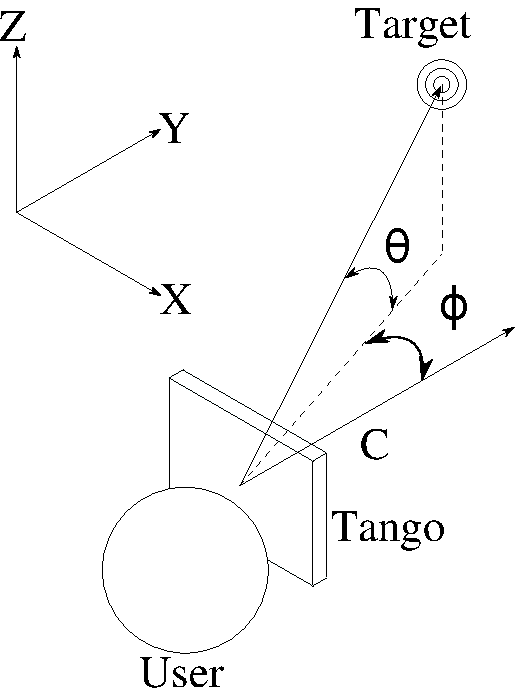
\includegraphics[width=0.4\columnwidth]{figures/camera_coordinate.pdf}
  \caption{A diagram showing the device's frame of reference and the target's pan and tilt angles.}\label{fig:cam-coords}
\end{figure}

The remainder of this paper is organised as follows: \cref{sec:lit-review} gives an overview of existing navigation systems and audio interfaces for people living with visual impairments.
\cref{sec:portable-navigation} discusses the navigation device's hardware and interface setup and describes how the target's position is conveyed to the user.
The experiment we conducted are explained in \cref{sec:experiments} and the results are presented and discussed in \cref{sec:results}. 
Finally, \cref{sec:conclusion} concludes this paper with a summary of the findings and comments on our future work. 

\section{Previous Work}\label{sec:lit-review}

\todo{chop up this section. Make anonymous}

Earlier attempts at improving a person with visual impairment's navigation experience involved outfitting the commonly-used walking cane with remote detection systems, such as sonar, radar and RFID tags, to transform a cane into an early-warning system~\cite{ulrich1997,marion2008batcane,faria2010electric,willis2005}.
Bluetooth tags and a smartphone can be used in a similar manner~\cite{sato2017navcog3}.
However, the expense and effort of maintaining such tags make them less attractive for wide-scale adoption.
Computer vision-based systems provide a good compromise between usability, cost and accuracy.
One increasingly popular solution is to use RGB-D depth sensing cameras, which are becoming increasingly accurate and cost-effective, to build a 3D image map of the environment, and guiding a user through it~\cite{lee2015, rodriguez2012obstacle}.
Alternatively, object recognition techniques can be used to detect various objects and landmarks, such as doors, staircases, etc., and communicate their relative location to the user~\cite{schauerte2012assistive, tian2013b, fiannaca2014headlock}, or use audio instructions to instruct a user with vision impairment to fully capture an object of interest~\cite{vazquez2012helping}. 

%Attempting to deliver a system that allows people with visual impairments to independently navigate and accomplish everyday tasks is not new; in fact, there are multiple commercial systems and research prototypes already available on the market.
%One approach that has been investigated is to outfit the existing white walking cane with various sensors, such as sonar, radar, motor encoders, etc.~\cite{ulrich1997, marion2008batcane} to warn the user of upcoming obstacles, instead of relying on haptic feedback from the impact between the cane and the obstacle.
%Another approach is to outfit a walking cane to act as a radio-frequency identification (RFID) antenna that can read a set of RFID tags placed at strategic locations around the environment at key spots or along a path~\cite{faria2010electronic, willis2005}.
%This modification to the traditional cane is more discreet than the systems mentioned earlier and has been shown to work well.
%Bluetooth tags and a smartphone can also be used in a similar manner~\cite{sato2017navcog3}.
%However, the major drawbacks here are the significant cost and effort of modifying existing infrastructure with RFID and Bluetooth tags and maintaining them to stay up to date with a changing environment.
%GPS-based systems~\cite{ran2004drishti, loomis2001navigating, kammoun2012navigation}, while cheap and reliable in outdoor environments, are not applicable in built-up urban areas and indoors where GPS signals are notoriously unreliable.
%Computer vision-based systems provide a good compromise between usability, cost and accuracy and have been the focus of much research recently~\cite{manduchi2014last}.
%One increasingly popular solution is to use RGB-D depth sensing cameras, which are becoming increasingly more accurate and cost-effective, to build a 3D image map of the environment, allowing a user to safely traverse through it~\cite{lee2015, rodriguez2012obstacle}.
%Another approach is to use vision-based object recognition techniques to detect various objects and landmarks, such as doors, staircases, etc., and communicate their relative location to the user~\cite{schauerte2012assistive, tian2013b, fiannaca2014headlock}, or use audio instructions to instruct a user with vision impairment to fully capture an object of interest~\cite{vazquez2012helping}. 

An important feature of user-centric systems is a human-machine interface (HMI) that enables effective two-way communication between the system and the user.
In previous surveys, researchers found that people with visual impairments prefer receiving instructions in the form of speech and haptic feedback cues~\cite{khoo2016multimodal, ross2000wearable, vazquez2012helping}.
However, haptic feedback modes typically have a lower bandwidth when compared to audio feedback and also require the user to wear a special device in order to transmit the signals effectively.
Work has also been done in translating a visual scene into non-visual formats, with so-called sensory substitution systems (e.g. `The Voice'~\cite{meijer2010}) and virtual audio reality (VAR) systems~\cite{frauenberger2003} reporting favourable results.
However, The Voice has a very steep learning curve that has proven to be a significant barrier to entry and with VAR systems, it is not clear how unknown environments, where markers have not yet been encoded, would be handled and described to the user. 

%Spatial audio has also been considered to convey the direction of a target.
Previous experiments have determined that people are able to find the location of a stationary sound source with an error of $\pm$\SI{35}{\degree}, in both the pan and tilt dimensions~\cite{zwiers2001spatial}, for both early-blind and normally-sighted people.
However, in~\cite{lewald2013exceptional, lessard1998early} it was found that the blind have a clear advantage in localisation accuracy over sighted people when presented with more complex tasks, such as targets in motion and narrow-band stimuli, with~\cite{lewald2013exceptional} reporting an average absolute localisation error of around \SI{10}{\degree} in the pan and tilt dimensions.
%Other authors found that the minimum difference in the spatial sound's angle for the user to be able to perceive movement is approximately \SI{1.7}{\degree}. 
%During these experiments, an audio speaker was physically manoeuvred to provide the participant with a spatialised sound tone~\cite{ashmead1998spatial}.
Researchers have used simulated spatialised audio to inform the user of the sound source's direction~\cite{holland2002audiogps, kammoun2012navigation, rebillat2009smart, menelas2010audio, wilson2007swan, zotkin2004rendering}.
In these works, a sound was played through a set of headphones and the source spatialised with a head-related transfer function (HRTF), tricking the listener into thinking the sound source was located at some arbitrary 3D location.
%Various audition techniques and methods were then used to guide the user along a path.
%Other authors have also provided a framework for evaluating the quality of this 3D sound in terms of its psychoacoustic properties~\cite{guastavino2004perceptual, nicol2014roadmap}.
There are also experimental results about how well users can find targets presented with spatial sound in the tilt and panning dimensions with normal headphones~\cite{katz2011spatial, zwiers2001spatial}, as well as work that has shown similar levels of localisation performance between normal and bone-conducting headphones in the pan dimension~\cite{macdonald2006spatial}.
However, to our knowledge no extensive work or experiments have been done to determine how well users respond to tilt adjustment instructions using a tone with \textit{varying pitch}, in particular when using bone-conducting headphones, and how changes to this tone's behaviour affects performance. 

\section{Portable Navigation System}\label{sec:portable-navigation}

\subsection{System Setup}

Our ultimate goal is to deliver a navigation system that can guide a user with visual impairments on the last leg of their journey, e.g.\ to a specific aisle and shelf in a shop, using only a mobile phone.
A large amount of data need to be translated from a visual form into a format that is useful to people with limited or no vision.
We therefore plan to use a combination of voice, audio and vibration cues to translate visual navigation data as effectively as possible and overcome the bandwidth limitation of the human ear. 
However, for this paper, we only considered the spatialised audio mode and its variation in pitch in order to determine its effectiveness in conveying a target's pan and tilt angles.

\begin{anonsuppress}
The system is based on a concept proposed in~\cite{bellotto2013, lock2017portable}, which uses a Google Tango device.
\end{anonsuppress}
The navigation system is based on a Google Tango tablet, an Android-based device that comes equipped with an RGB-D cameras to sense colour and depth.
It combines an inertial measurement unit with powerful and robust landmark recognition and image processing algorithms to localise itself in real-time.
An added benefit of this platform is its familiar, compact form-factor which will help overcome the hurdle of user-acceptance and usability.
We also use a set of bone-conducting headphones (see \cref{fig:tango-headphone}) that are placed externally on a user's head so that the system does not occlude the perception of real-world sounds and does not interfere with a user's normal hearing function.
%In the future, we will use multiple feedback modes to provide the user with navigation and obstacle avoidance instructions.

A diagram of the experimental system pipeline is shown in \cref{fig:pipeline}, where the arrows indicate the direction of the flow of information.
When the user taps the Tango's screen, a new virtual target is generated and its coordinates are sent to the audio generation module, along with the device's current position and orientation.
The audio generator then produces a tone based on the difference between the device and target's positions and sends it to the audio output channel, which plays it back to the user.
The WiFi recording module is constantly monitoring the different parameter values of the device and target's positions, as well as the system's output, and records it to a remotely stored datafile. 

\begin{figure}
  \centering
  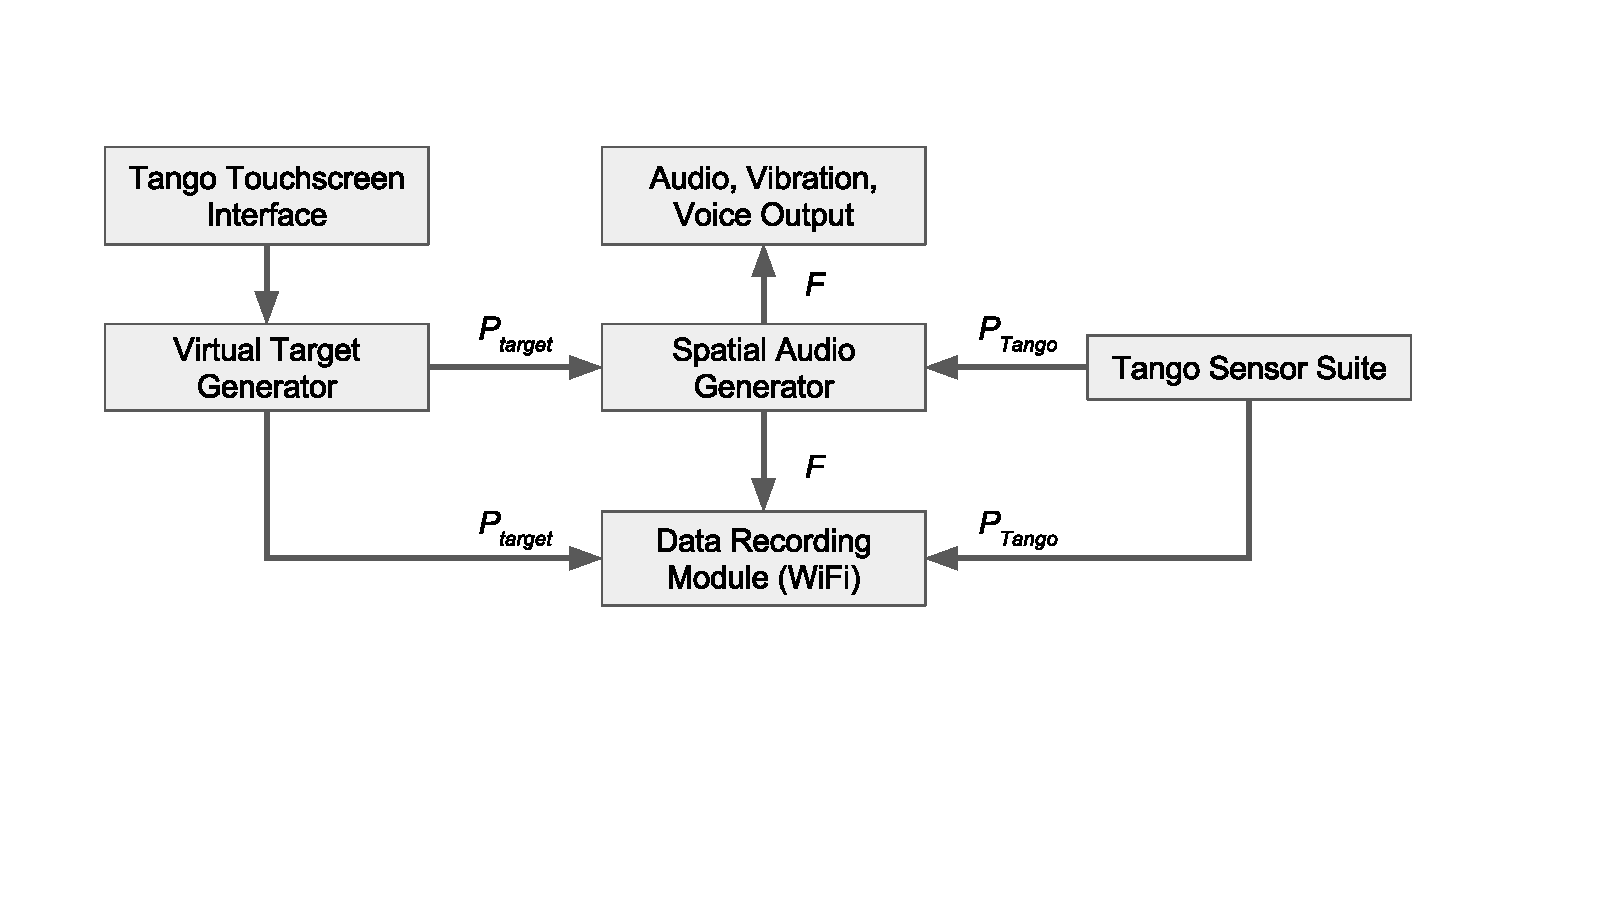
\includegraphics[clip=true, trim=0 120 80 50, width=1.0\columnwidth]{figures/pipeline.pdf}
  \caption{A diagram of the individual system components and their communication pipelines. $F$ indicates a feedback signal and $P$ a pose signal. }\label{fig:pipeline}
\end{figure}

\subsection{Audio Interface}

%For the series of experiments performed in this work, only the audio feedback mode was used to interface with the user.
The audio component is responsible for conveying the 2D position of a target on the vertical plane, showed in \cref{fig:cam-coords}, in terms of pan and tilt angles.
%In future system iterations, the distance to a target can be rendered by adjusting the audio signal's amplitude as a function of the distance.
The audio signal is a continuous $\sim$\SI{10}{\hertz} sinusoidal sound wave that is played to the user through bone-conducting headphones.
We use a sinusoidal wave here because it is relatively simple to manipulate and analyse and will be replaced by a richer, more natural tone at a later stage. 

The audio is spatialised in the pan dimension using the OpenAL\footnote{http://openal.org} sound library's HRTF, while the tilt angle is conveyed by varying the audio tone's pitch.
We use this approach because the external set of bone-conducting headphones plays the sound through a user's cheekbones instead of their outer ears, bypassing the ears' pennae that provide the ability to localise elevated sound sources~\cite{roffler1968factors, algazi2001elevation}.
This makes an HRTF less effective in conveying the target's elevation and therefore needs to be conveyed using another method; by varying the tone's pitch in this case.
The difference between the target's angular position and the device's angular orientation are used to generate the audio signals. 

\subsubsection{Pan Direction}

The pan angle ($\phi$) describes the angle which the user needs to rotate the camera vector, $C$, around the $z$-axis shown in \cref{fig:cam-coords}, i.e.\ how far the target is to the left or right of the user.
We use an HRTF to add a spatial element to the audio tone that is played to the user, placing the sound source at the target's location. 
Humans determine a sound source's pan direction by subconsciously analysing the inter-aural time difference (IID) between a sound reaching both of your ears: the greater the IID, the greater the perceived angular distance to the sound source~\cite{wightman1992dominant}.

We implement OpenAL's default HRTF, based on the MIT's KEMAR dataset\footnote{sound.media.mit.edu/resources/KEMAR.html}, to generate a sinusoidal sound wave based on the difference between the user and target's positions.
The library takes position values as input and outputs a tone based on the angle between the two position vectors. 

\subsubsection{Tilt Direction}

The system adjusts the tone's pitch ($f$) to convey the target's tilt angle ($\theta$) w.r.t.\ $C$, as shown in \cref{fig:cam-coords}. 
Here, a high pitch means the target is above $C$ (i.e.\ the user should look up) and a low pitch means the target is below $C$ (the user should look down).
This high/low association scheme is chosen because humans naturally associate high-pitched sounds with higher objects and lower-pitched noises with lower objects~\cite{pratt1930spatial, blauert1997spatial}.
We use a logarithmic, octave-based gain function for the pitch, since an increase in octave provides a distinct perceptible change while keeping the timbre roughly constant~\cite{shepard1964circularity}.

We wish to determine how the gradient of the pitch gain as a function of $\theta$ (i.e.\ $m = \frac{df}{d\theta}$) affects a user's performance, e.g.\ does a greater $m$ lead to an increased target acquisition rate?
For this we select 3 different pitch settings, referred to henceforth as $m_l$, $m_m$ and $m_h$ for the smallest, middle and highest gain gradients respectively. 
To find these gradients, we set the maximum and minimum limits for $\theta$ and the maximum and minimum frequencies for $f$ for each respective setting.
Furthermore, for the sake of consistency and between the different settings, each gradient generates the same pitch when $C$ is level with the target's tilt. 

After practical tests with the device and headphones, we set the neutral, on-target tone to $f_{512} =$ \SI{512}{\hertz} for its audibility.
For $m_l$, we set $f_{max}$ and $f_{min}$ to 1 octave higher and lower than $f_{512}$, giving limits of \SI{1024}{\hertz} and \SI{256}{\hertz} respectively.
For $m_m$, the $f_{max}$ and $f_{min}$ are set to 2 octaves higher and lower than $f_{512}$ (\SI{2048}{\hertz} and \SI{128}{\hertz}) and $m_h$ to 3 octaves higher and lower (\SI{4096}{\hertz} and \SI{64}{\hertz}).
We selected these limits for practical reasons, given the fact that the bone conducting headphones we use have low volume gain at the frequency spectrum extremes, making it difficult to hear. 
The values of $m_l, m_m, m_h$ are visualised in \cref{fig:pitch-gain}.

\begin{figure}
  \centering
  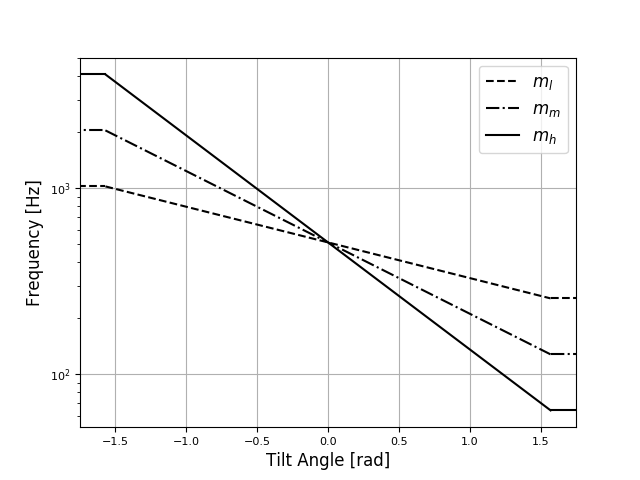
\includegraphics[width=1.0\columnwidth]{figures/pitch_gain_functions.png}
  \caption{The pitch gain functions for the 3 different gain settings. }\label{fig:pitch-gain}
\end{figure}

We set the range of angles the system can convey to $[-\frac{\pi}{2}; \frac{\pi}{2}]$; anything outside this range implies that the target is behind the user and was not considered in this series of experiments. 
The \SI{0}{\radian} position is directly in front of the user.
With these limits, $f$ can be determined with \cref{eq:frequency}, where $m$ is the given setting's gradient, $\frac{df}{d\theta}$, and $c$ can be found using the current setting's pitch and angle limits.

\begin{equation}\label{eq:frequency}
  f(\theta) = 2^{-m\theta + c}
\end{equation}

\section{Target Search Experiment}\label{sec:experiments}

We conducted a set of experiments to evaluate the audio interface's effectiveness at driving a user to point the camera at a target in the pan and tilt dimensions.
Furthermore, we wish to see how changes to $\frac{df}{d\theta}$ affect a user's performance.

We recruited 2 groups of participants for the experiments.
Group $G1$ consists of 42 young adults (mostly students) with healthy eyesight, with 10 males and 32 females being $20\pm1.5$ years old on average.
This group was blindfolded throughout the experiment and forms the bulk of the participant population.
Group $G2$ is made up of 3 legally blind adults with varying levels of vision limits (3 males, average age of $40\pm8$ years). 
This group makes up less than 10\% of the total population, but provided valuable subjective feedback that will help improve the system before evaluating it with a larger group of people with vision impairments. 
All participants joined the experiment on a voluntary basis with written consent and none have any other impairments that affects their interpretation of the audio guidance cues.

For the experiment, the participants were given a Tango tablet device, running an app written for this experiment, and a pair of AfterShockz Sportz3' bone conducting headphones (both pictured in \cref{fig:tango-headphone}) and were blindfolded where appropriate.
The app generates a virtual target, one at a time and a constant \SI{2}{\metre} from the participant, and uses the device's measurements to determine $\phi$ and $\theta$.
These angles are then used to generate and present the user with the audio signal to direct them to the target. 
As the participant rotates the camera, $\phi$ and $\theta$ are adjusted and the audio signal changes according to reflect the changes.
When a participant was satisfied that they were on target, they tapped the screen which generated a new target target which they were then directed to. 
Each participant was given 28 targets in total that were randomly generated and equally spread across 4 quadrants to avoid clustering. 
After the 28 targets were found, the gradient setting ($m$ in \cref{eq:frequency}) was adjusted and the experiment was repeated. 
The order in which the gradient setting was changed for each participant was randomised to minimise any the learning effect.
The app streams various data on the current device and target poses to a laptop computer via a WiFi connection in real-time. 
Before the experiment session started, each participant was given some time to familiarise themselves with the device and the audio tone and was given the oppertunity to learn what the $f_{512}$ `on-target' and on-centre tone sounds like that will confirm that they are level with the target.

The measure of performance here is the accuracy with which a user points the camera towards a target.
The accuracy is taken as the angular difference between the device's and target's poses at the time the participant tapped the screen and a smaller error would indicate more accurate results.
The pan and tilt results are separated to understand the effect of changing the gradient setting has on either dimension's accuracy.
To minimise the speed/accuracy biases in the results, we asked the participants to focus on finding the targets as well as they could without worrying about the time it took.  

%We performed a set of experiments with our audio interface to determine its effectiveness at directing a user to adjust a camera's $\phi$ and $\theta$ to point it to a target.
%The results from the experiments allow us to better understand how the users respond to different settings for the spatial audio feedback stimulus and use them to improve and optimise the behaviour of the feedback modes in our portable navigation aid.

%The participants were given time before the experiments to familiarise themselves with the device and the tones it emits, as well as what the $f_{512}$ `on-target' tone sounds like.
%We also tested the system with 3 legally blind participants and compared their data to the blindfolded dataset.
%These latter experiments in particular provided us with valuable subjective feedback that can be used to improve future iterations.

%For the experiments we used two groups of participants, with one ($G1$) including 42 sighted and blindfolded participants and the other ($G2$) 3 legally blind volunteers with varying degrees of vision impairment. 
%They performed a series of experiments using our system with a pair of `AfterShockz Sport3' bone-conducting headphones.
%The participants were recruited on a volunteer-basis and consisted of a diverse group of undergraduate students and professionals with ages ranging between 17 and 40 years ($\mu=22\pm3.5$ years, 13 male, 32 female) and did not not have significant hearing issues or any other disability that could affect the experiment.

%We are only evaluating the interface in the pan and tilt dimensions and the 3D targets are therefore generated at a constant distance of \SI{2}{\metre} from the participant.
%Throughout the experiments, various parameters of the targets and participants were recorded and streamed in real-time to a laptop computer via a WiFi connection.

%For the experiment, the participants were blindfolded where necessary and given a Tango device running an app purpose-written for this experiment.
%When started, a set of virtual targets were presented one at a time to the participant on the device.
%Then, depending on the direction the participant was currently pointing the camera relative to the target's position, the Tango generated and played a tone via the bone-conducting headphones to indicate the pan and tilt angle adjustment required to point the camera to the target. 

%Once the participant pointed the camera toward where they thought the target was located, they had to tap the screen to confirm the target's perceived location at which point a new target was presented and the search-process was repeated.
%28 targets were presented to each participant per run.
%The positions of these targets were randomly generated and equally spread across the 4 quadrants on the vertical plane to prevent a clustering of targets at the same location.
%After every experiment run, the gradient ($m$ in \cref{eq:frequency}) was adjusted to make the pitch increase at a lower or higher rate.
%This was done to see whether, for example, a more rapid increase in pitch would help the participant find the target faster or more accurately.

%To minimise any speed/accuracy trade-off bias in the results, we asked the participants to search for the targets without placing particular emphasis on accuracy or time. 
%The order in which the settings were set for each participant was randomised in order to minimise any learning effect the participant population might display between each experiment. 

%In this case, the system's measure of performance is given by the target acquisition accuracy.
%The accuracy is given as the difference between the device's orientation at the time the participant confirmed they were on target, and the target's actual angular position.
%We separate the results of the tilt and pan dimensions in order to determine how the different pitch settings affect pointing accuracy. 

\section{Results and Discussion}\label{sec:results}

The results for the participants in $G1$ given if the 2D histograms in \crefrange{fig:err-results-lo}{fig:err-results-hi}, where the pan error is on the abscissa and the tilt error on the ordinates.
A set of box-plots of the angular errors' median and standard deviations are given in \crefrange{fig:err-boxplot-median}{fig:err-boxplot-std} for the $m_l, m_m$ and $m_h$ settings. 
The results for $G1$ are summarised in \cref{tab:results}.

\begin{figure}
  \centering
  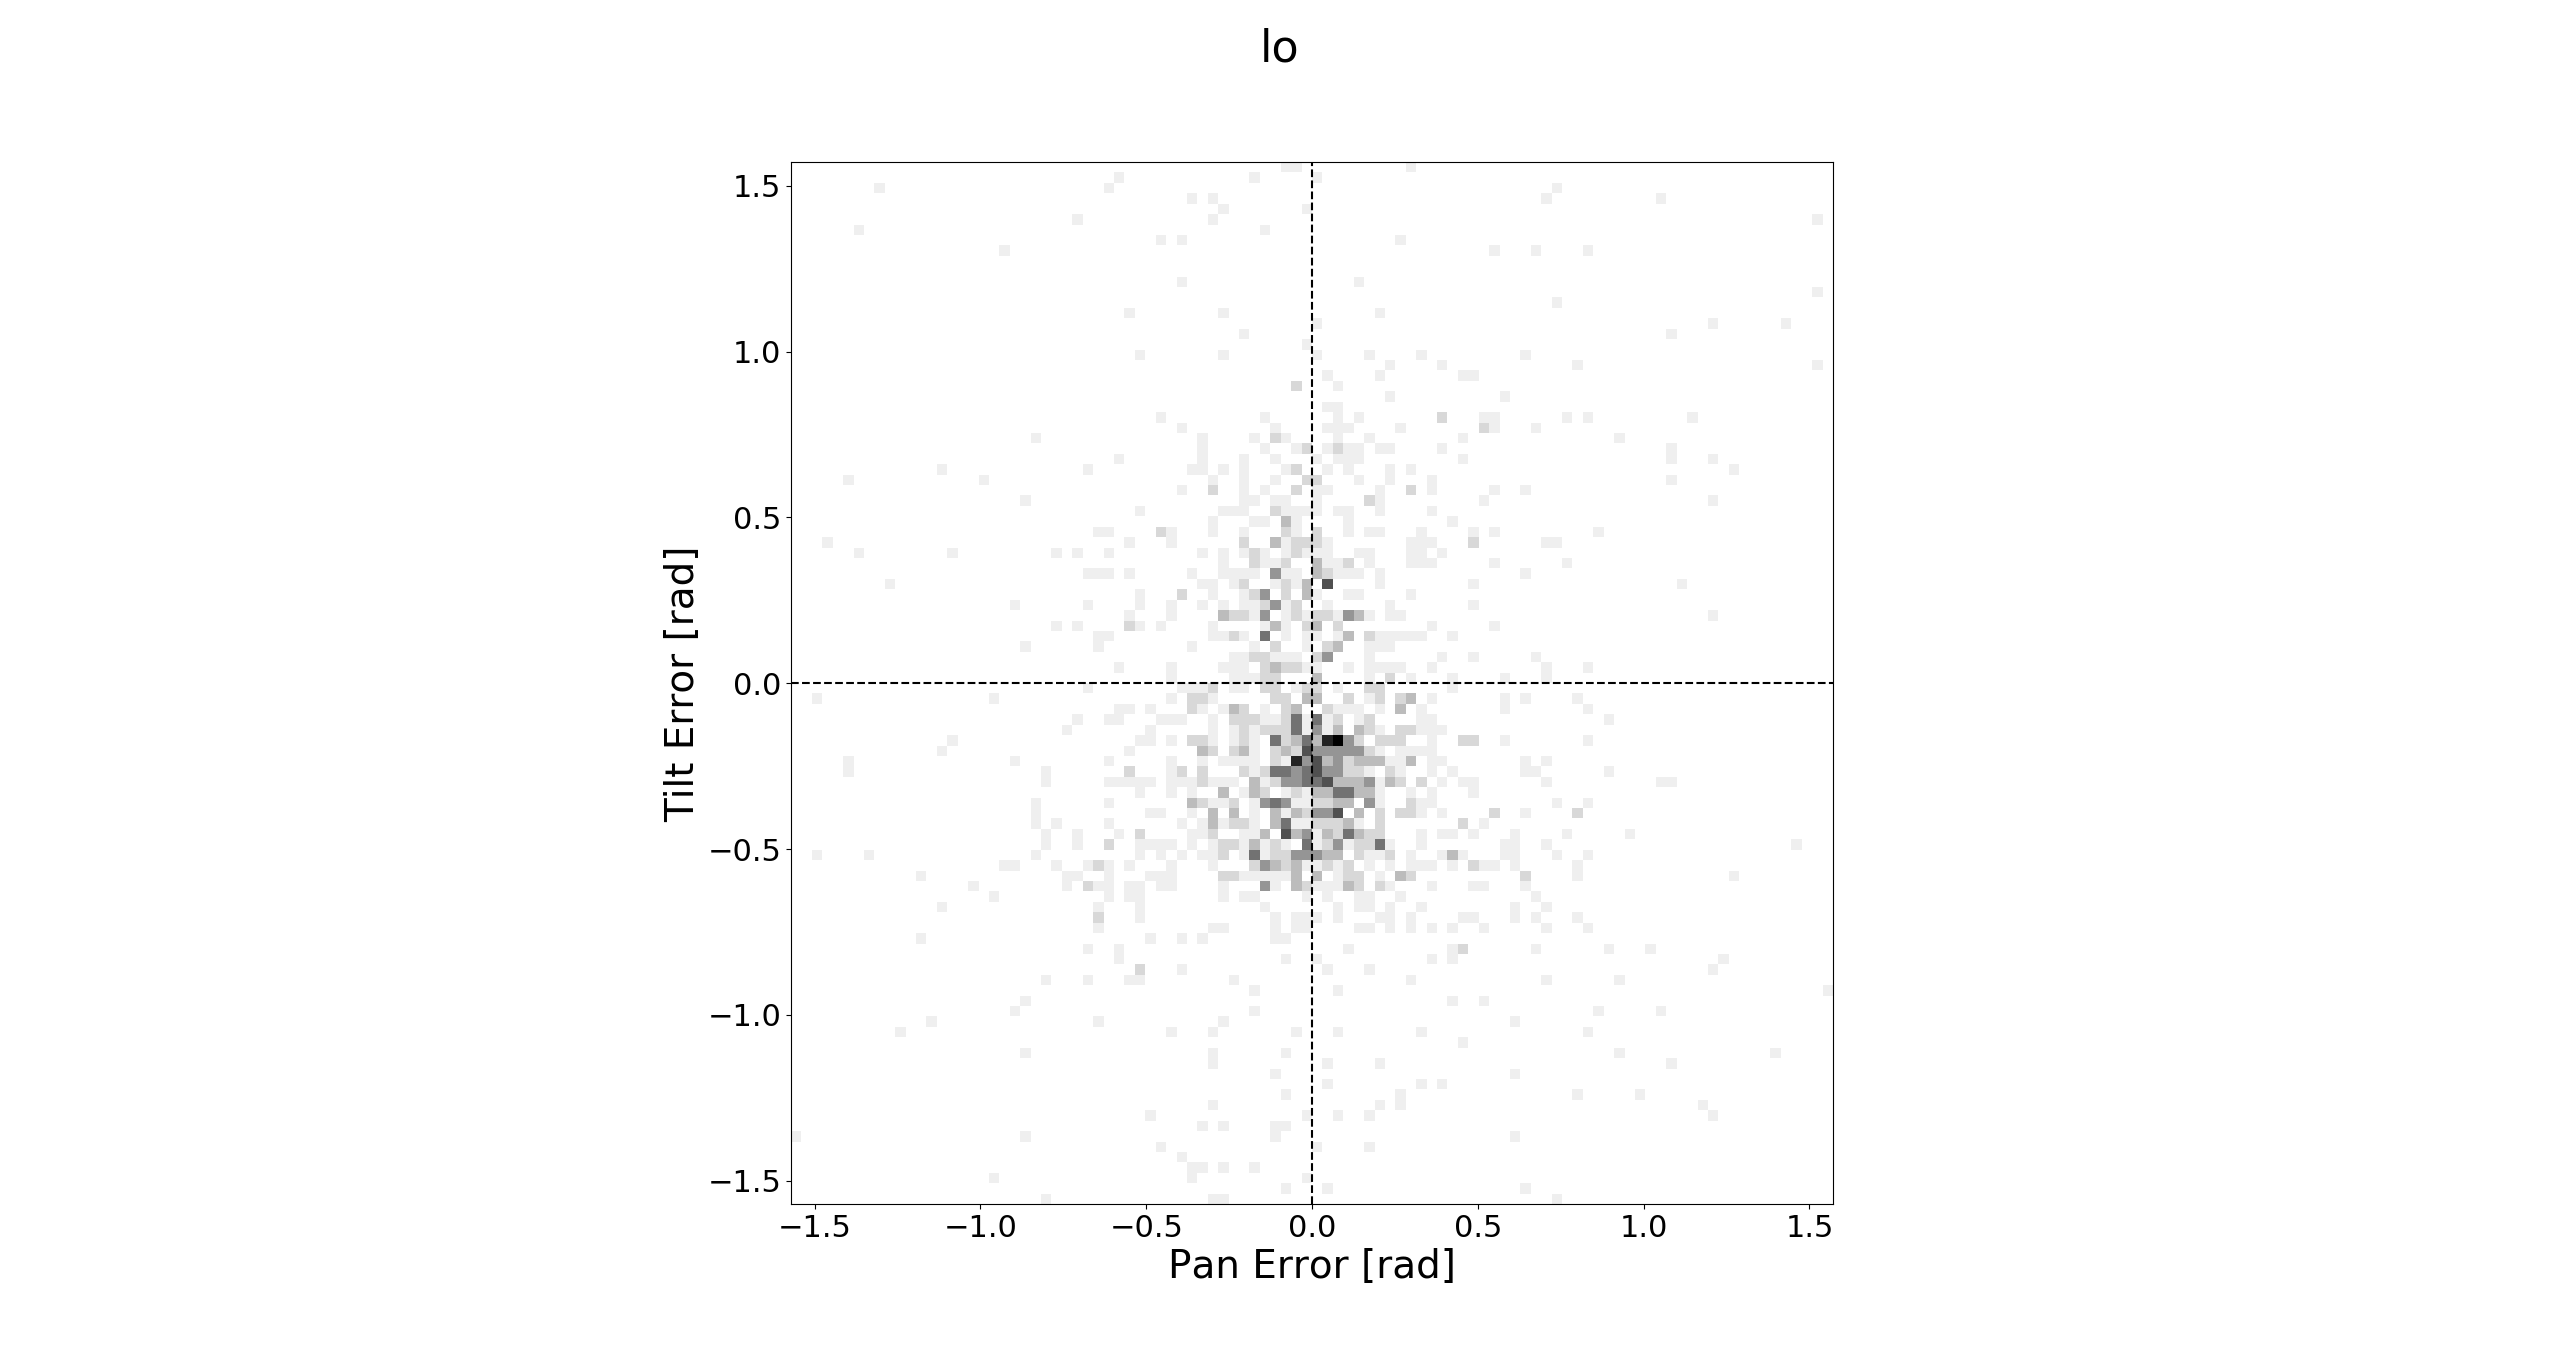
\includegraphics[clip, trim=450 0 450 110, width=0.8\columnwidth]{figures/err_lo.png}
  \caption{Angular error data for $G1$ and the $m_l$ setting. }\label{fig:err-results-lo}
\end{figure}

\begin{figure}
  \centering
  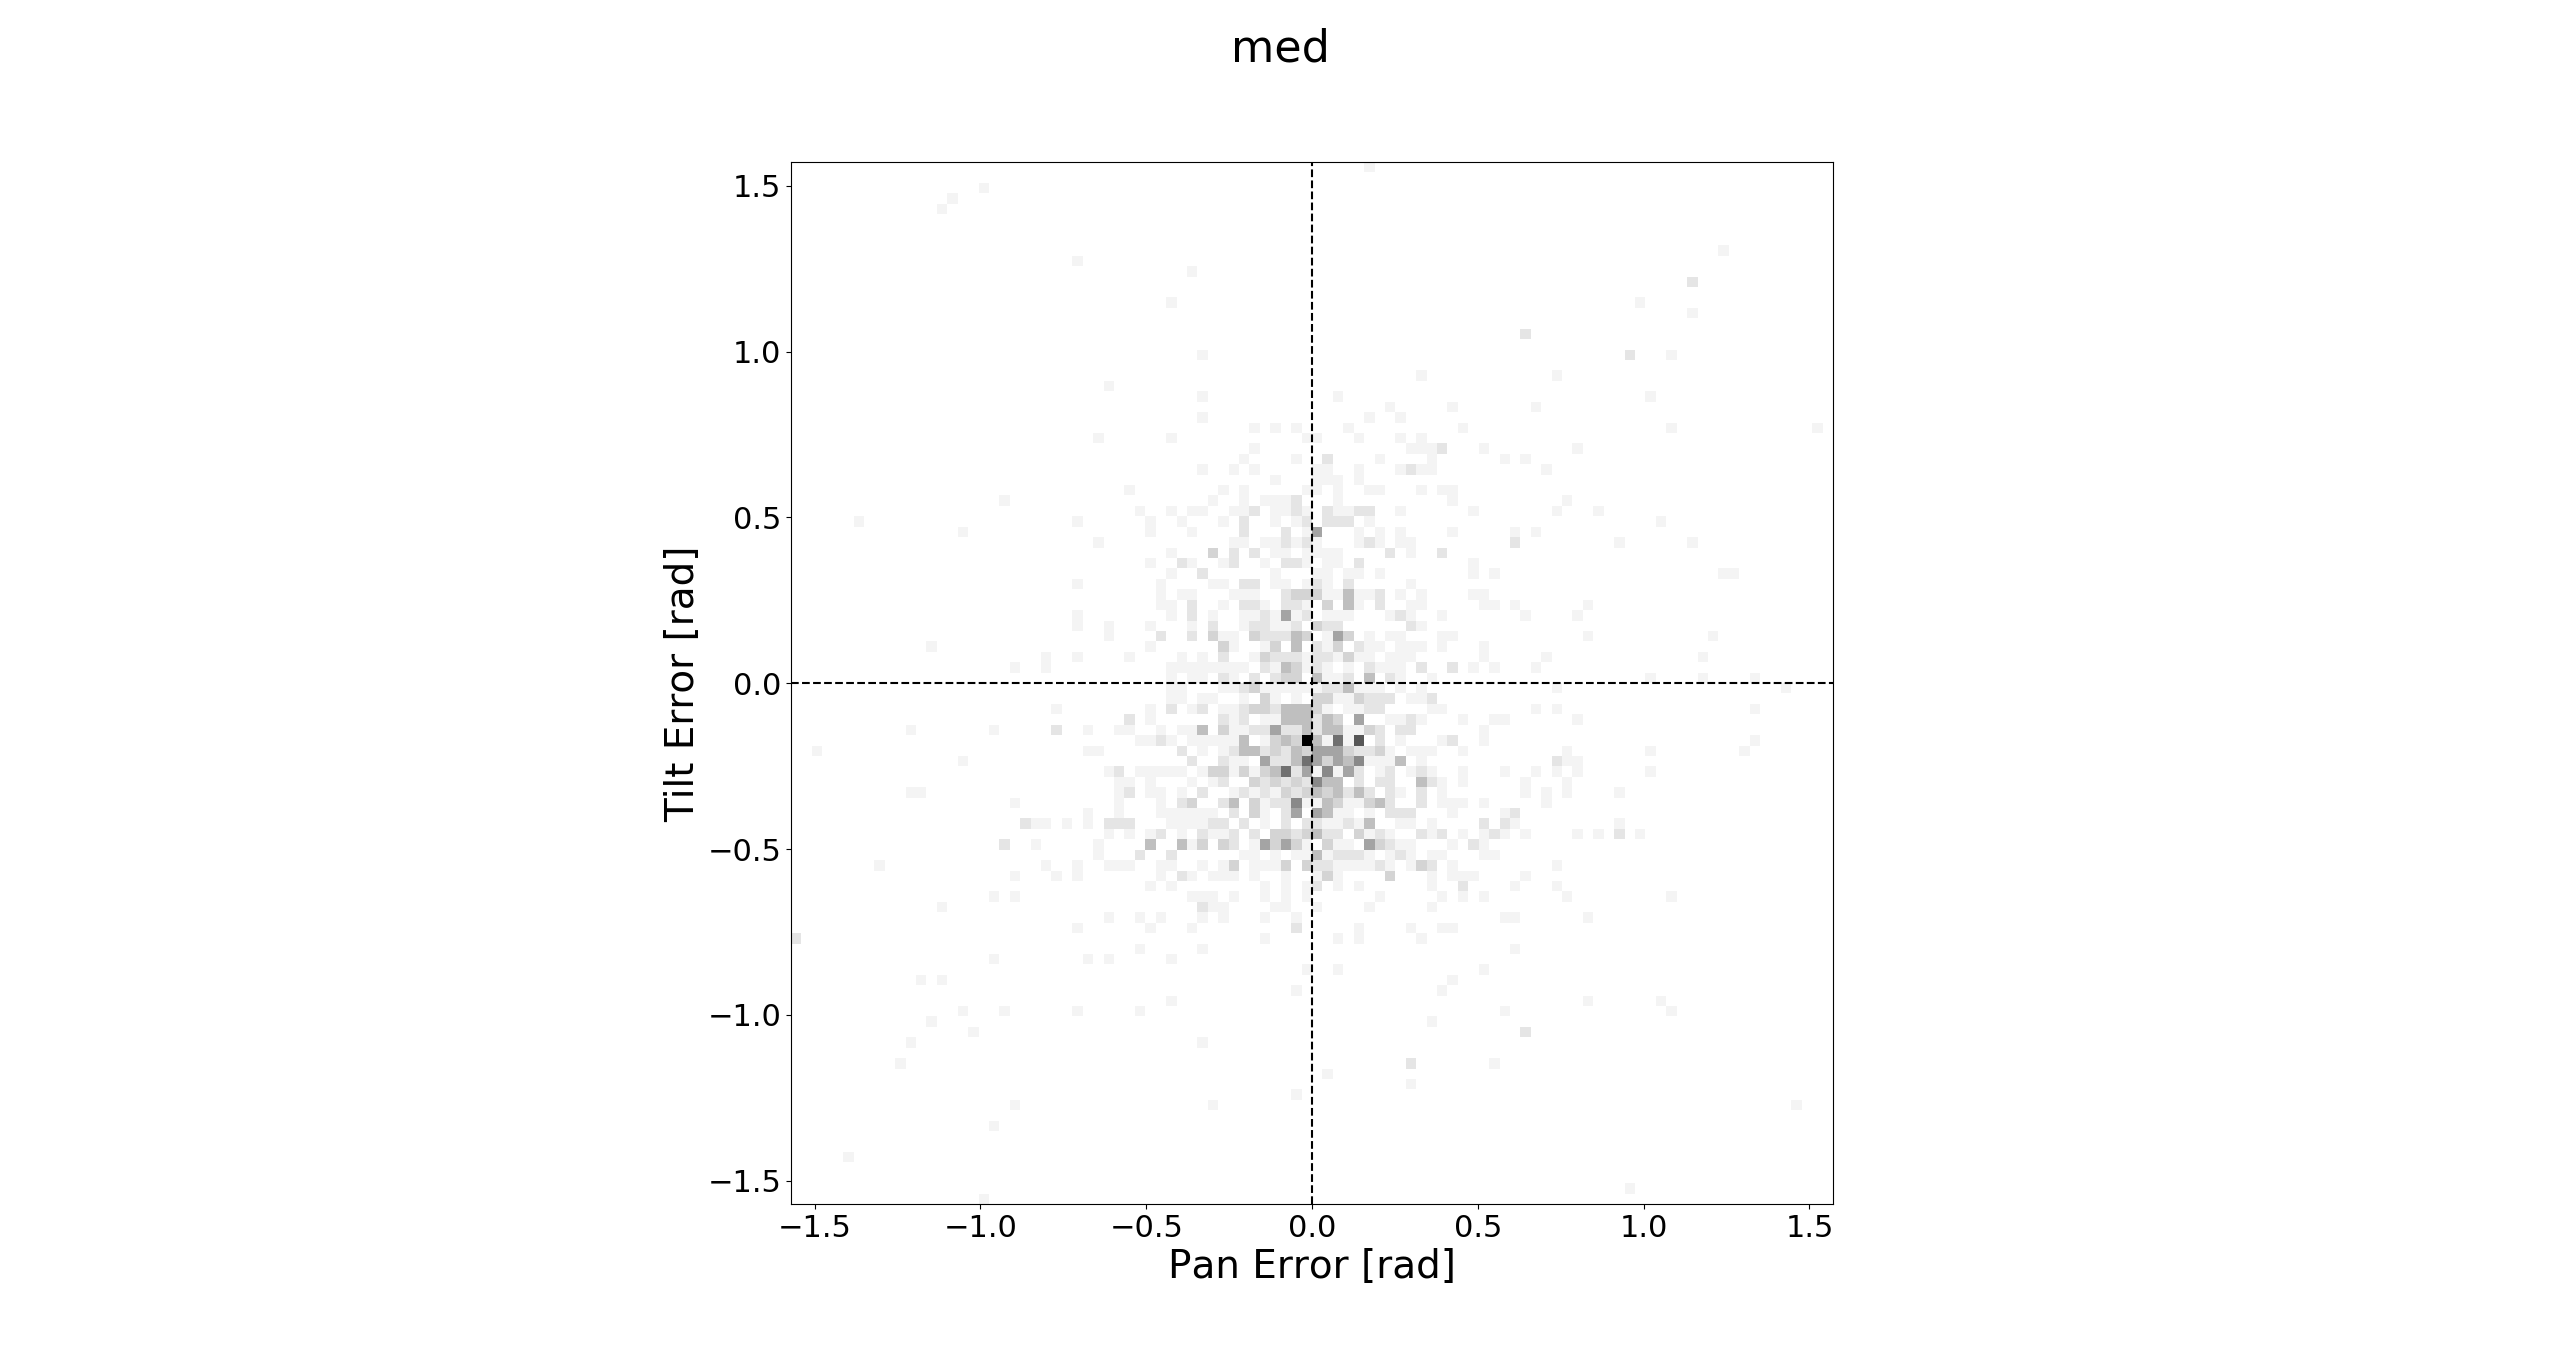
\includegraphics[clip, trim=450 0 450 110, width=0.8\columnwidth]{figures/err_med.png}
  \caption{Angular error data for $G1$ and the $m_m$ setting. }\label{fig:err-results-med}
\end{figure}

\begin{figure}
  \centering
  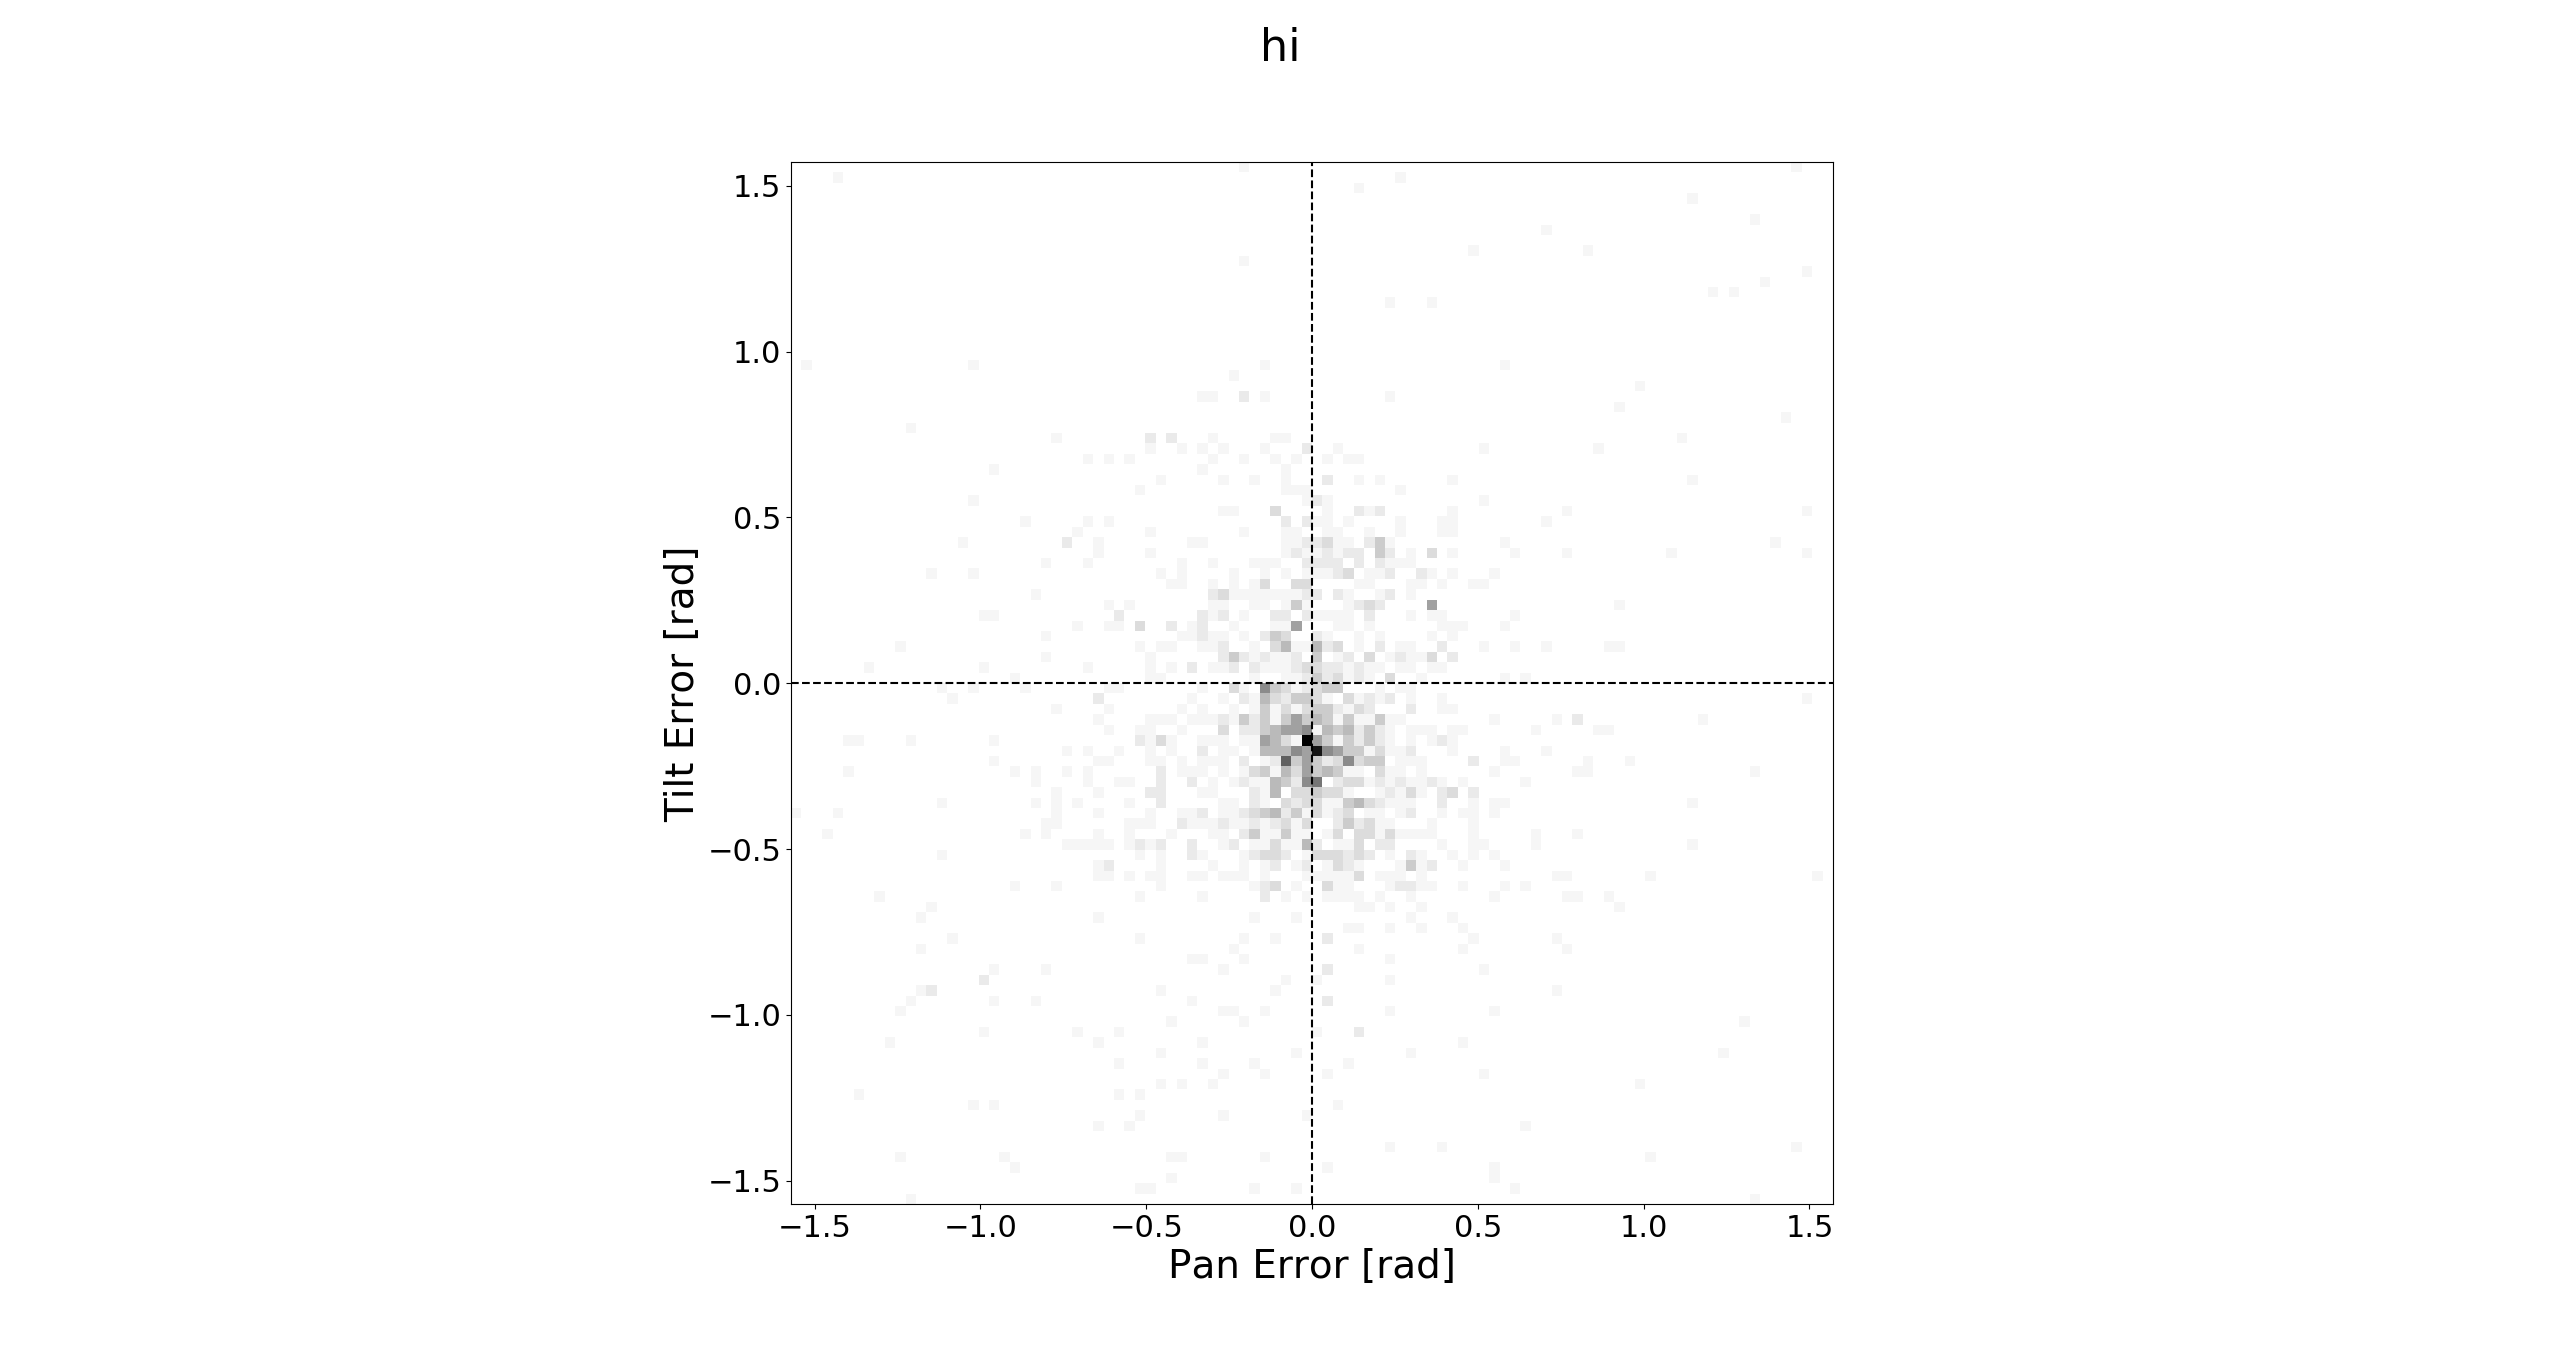
\includegraphics[clip, trim=450 0 450 110, width=0.8\columnwidth]{figures/err_hi.png}
  \caption{Angular error data for $G1$ and the $m_h$ setting. }\label{fig:err-results-hi}
\end{figure}

\begin{figure}
  \centering
  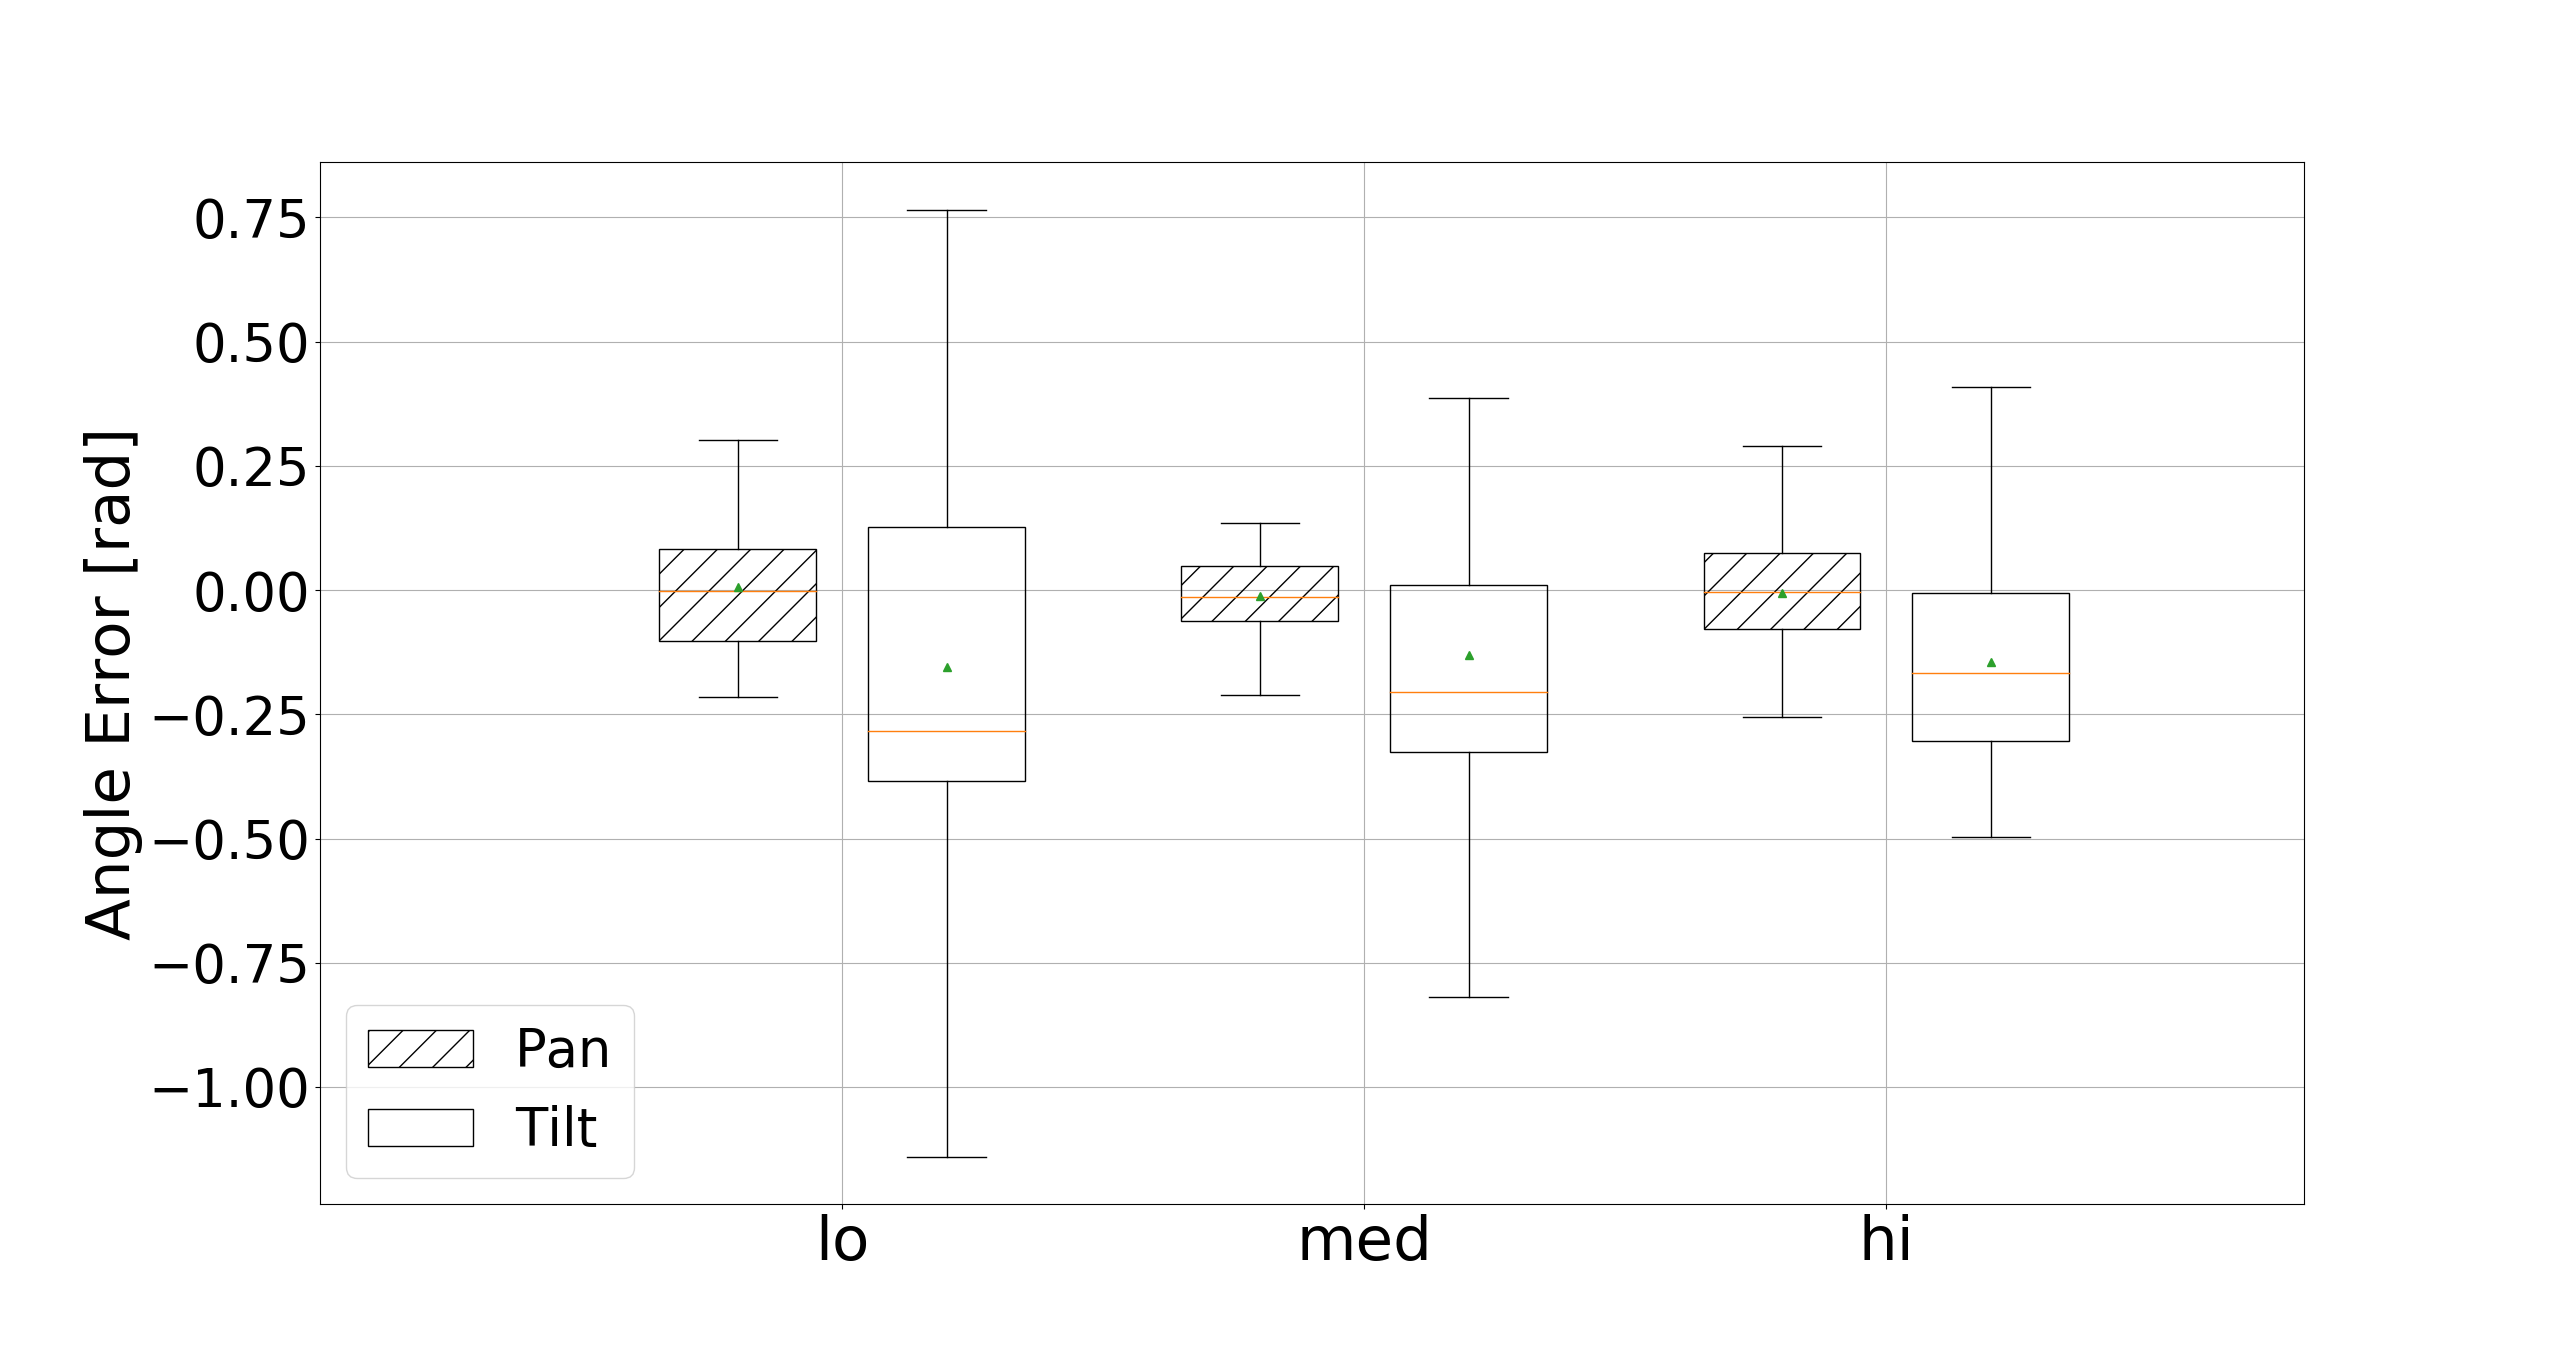
\includegraphics[clip, trim=20 -70 100 100, width=0.8\columnwidth]{figures/err_boxplot_medians.png}
  \caption{Error medians for $G1$.}\label{fig:err-boxplot-median}
\end{figure}

\begin{figure}
  \centering
  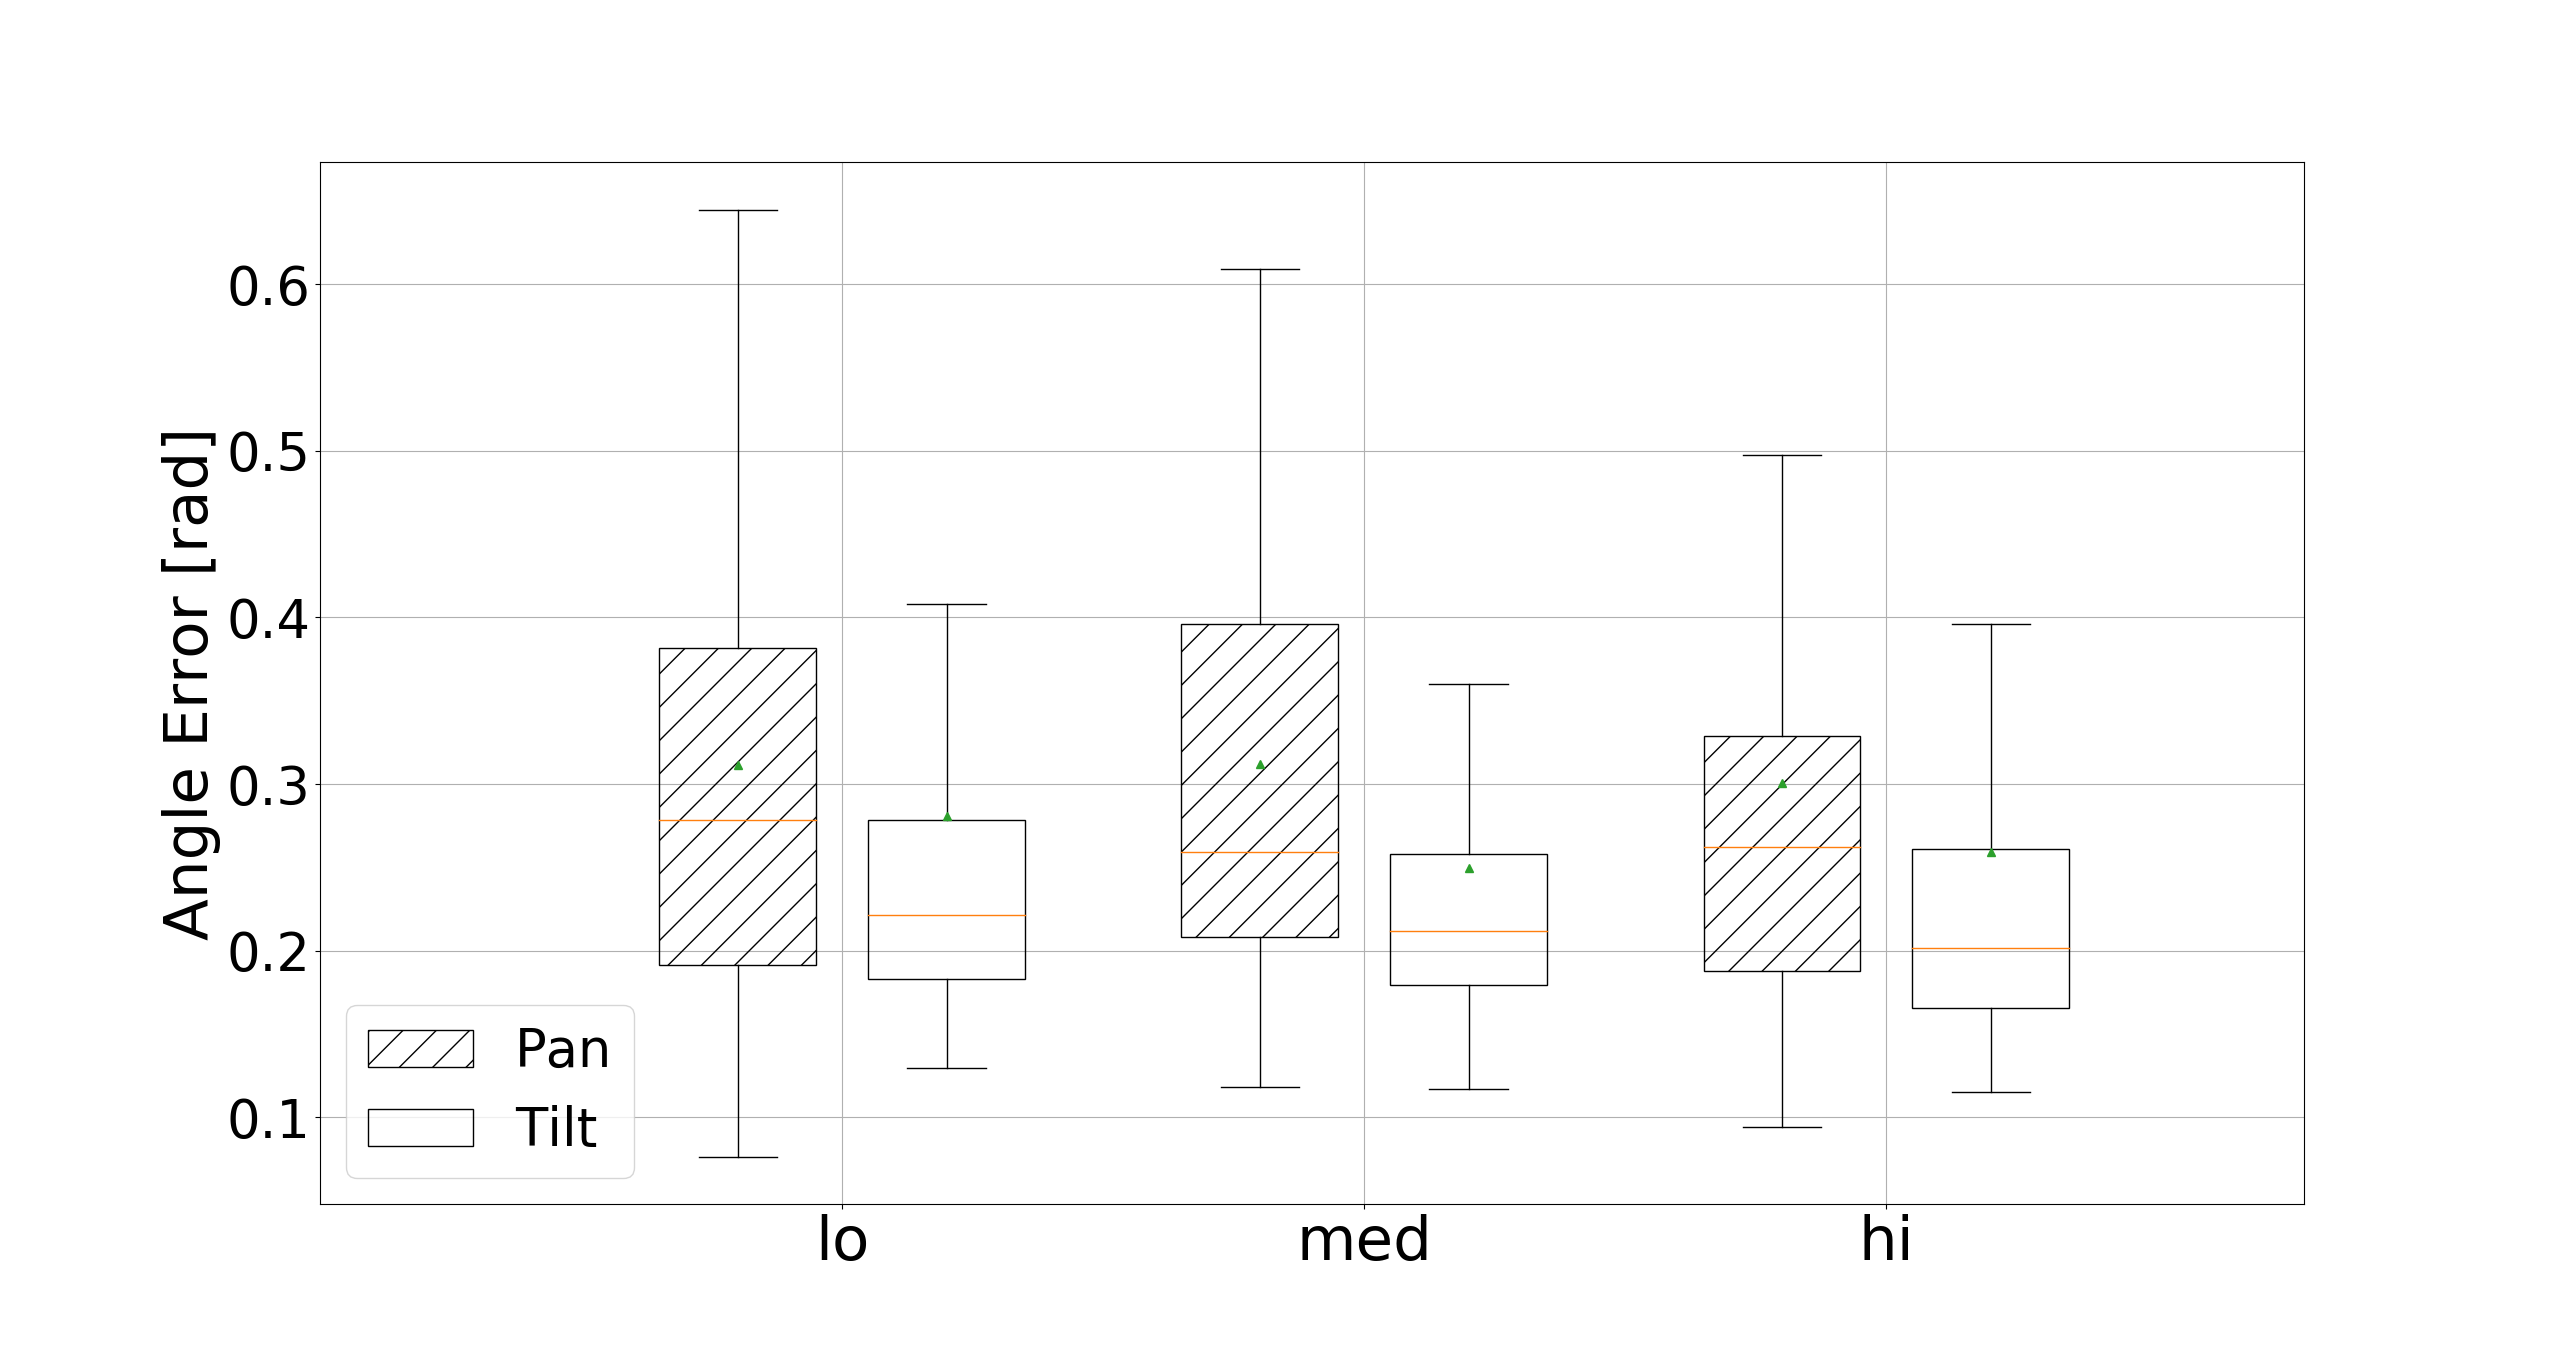
\includegraphics[clip, trim=80 -70 100 0, width=0.8\columnwidth]{figures/err_boxplot_std.png}
  \caption{Error standard deviations for $G1$.}\label{fig:err-boxplot-std}
\end{figure}

\begin{table}
  \centering
  \caption{A table of the pan and tilt angular error results collected from $G1$. The results include the absolute average error ($\mu_{abs}$), average error ($\mu$) and standard deviations ($\sigma$) given in radians, as well as the Spearman ($R$) correlation scores.}\label{tab:results}
  \begin{tabular}{llcccc}
    \toprule
    \multicolumn{2}{c}{} & $\mu_{abs}$ & $\mu$ & $\sigma$ & $R$ \\\midrule
         & $m_l$ & 0.23 & -0.02 & 0.32 & 0.75 \\%\cmidrule{2-6}
    Pan  & $m_m$ & 0.21 & -0.01 & 0.28 & 0.77 \\%\cmidrule{2-6}
         & $m_h$ & 0.22 & -0.05 & 0.31 & 0.75 \\\midrule
         & $m_l$ & 0.40 & -0.14 & 0.46 & 0.38 \\%\cmidrule{2-6}
    Tilt & $m_m$ & 0.32 & -0.12 & 0.36 & 0.48 \\%\cmidrule{2-6}
         & $m_h$ & 0.34 & -0.16 & 0.39 & 0.55 \\
    \bottomrule
  \end{tabular}
\end{table}

\subsection{Pan Results}


\crefrange{fig:err-results-lo}{fig:err-results-hi} and the median and mean points from the box-plots in \crefrange{fig:err-boxplot-median}{fig:err-boxplot-std} show that the data in the pan dimension is approximately normally distributed around zero.
However, $p$-scores below the critical 0.05 level from the Shapiro-Wilkes test and inspection of the quantile-quantile (Q-Q) plots do not give enough confidence to consider the data as normally distributed and we therefore analyse the data through non-parametric techniques. 

For the data collected from $G1$, there is a strong linear correlation between the participants' guesses and the targets' true pan angles, shown by the high Spearman correlation scores of approximately 0.75 ($p < 0.01$) for all of the datasets, with the $m_m$ setting displaying the marginally best result of 0.77.
The 3 settings have similar average errors and standard deviations, with the $m_m$ setting again producing the marginally best results with the smallest average error and standard deviation.
However, the differences are relatively small (approximately 6\%) and are not significant enough (Friedman test $p \gg 0.05$) to conclude that the pitch gradient has an effect on the target acquisition accuracy performance in the pan dimension. 

The data collected from $G2$ follow a similar trend to that of $G1$: the error in the pan dimension is centred around \SI{0}{\radian} with similar standard deviations across all 3 settings.
These results are summarised in \cref{tab:vi-results}.
Unfortunately, not enough samples could be collected to draw any final conclusions.
However, these results are in line with results from previous work~\cite{zwiers2001spatial}, indicating that the groups with partial and normal eyesight respond with similar levels of accuracy to spatialised sound when presented with simple tasks. 
In addition, they also confirm that a participant's target search capability in the pan dimension is robust to the changing pitch for the target's tilt angle which is a useful result in support of the effectiveness of our audio interface.

\begin{table}
  \centering
  \caption{A table summarising the target search results of the participants in $G2$ (P1 - P3). The results include the average error ($\mu$) and standard deviation ($\sigma$), given in radians in the pan and tilt dimensions.}\label{tab:vi-results}
  \begin{tabular}{llcccccc}
    \toprule
    \multicolumn{2}{c}{} & \multicolumn{2}{c}{$m_l$} & \multicolumn{2}{c}{$m_m$} & \multicolumn{2}{c}{$m_h$} \\
    \multicolumn{2}{c}{} & $\mu_l$ & $\sigma_l$ & $\mu_m$ & $\sigma_m$ & $\mu_h$ & $\sigma_h$ \\\midrule
	 & P1 &  0.25 & 0.44 &  0.21 & 0.45 &  0.29 & 0.40 \\% \cline{2-8}
    Pan  & P2 &  0.18 & 0.85 &  0.05 & 0.49 & -0.08 & 0.32 \\% \cline{2-8}
	 & P3 & -0.10 & 0.67 & -0.08 & 0.61 & -0.08 & 0.50 \\ \midrule
	 & P1 & -0.17 & 0.21 & -0.10 & 0.2  & -0.25 & 0.21 \\% \cline{2-8}
    Tilt & P2 & -0.87 & 0.26 & -0.05 & 0.21 & -0.15 & 0.18 \\% \cline{2-8}
	 & P3 & -0.57 & 0.31 & -0.57 & 0.45 & -0.38 & 0.39 \\% \hline
    \bottomrule
  \end{tabular}
\end{table}

\subsection{Tilt Results}\label{sec:tilt-results}

The ordinates in \crefrange{fig:err-results-lo}{fig:err-results-hi} also show the results recorded during the experiment with $G1$ in the tilt direction.
A set of box-plots are given in \cref{fig:err-boxplot-median} to show the average tilt error between the participants in $G1$'s guesses and the targets' true positions.
All of the results are summarised in \cref{tab:results}. 
The data here are also considered not normally distributed following inspections of the Q-Q plots and Shapiro-Wilkes test results and are analysed accordingly.

We found that there is reasonably significant correlation between the participants' guesses and the actual locations of the targets, shown by moderate Spearman correlation scores of approximately 0.38 for \emph{lo}, 0.48 for \emph{med} and the \emph{hi} gradient giving the strongest R-scores of the 3 with a score of 0.55 ($p < 0.01$ for all 3 settings).
This indicates that the varying pitch is working as expected and the participants are generally interpreting the cues correctly. 

The average errors of the datasets are relatively close to one another, with the $m_l$ setting producing the largest absolute error and standard deviation at \SI{0.40}{\radian} and \SI{0.46}{\radian}.
The $m_m$ and $m_h$ settings have similar absolute errors of \SI{0.32}{\radian} and \SI{0.34}{\radian} respectively.
This is in line with the correlation scores, with $m_l$ giving a worst result and $m_h$ giving the best results overall, with highest correlation score and relatively low absolute angular errors and standard deviation, marginally beating $m_m$. 

We use the Friedman test on the medians of the data to better understand the difference differences between the datasets.
We use the median values here since the data are not normally spread and there is significant noise within the data which may contaminate the mean values.
The Friedman test indicates a statistically significant difference between the 3 settings ($p < 0.01$).
A post-hoc analysis with a Wilcoxon signed rank test and a critical threshold with a Bonferroni correction applied for the 3 settings ($\alpha=0.016=\frac{0.04}{3}$) shows that both the $m_m$ and $m_h$ settings are significantly different than the $m_l$ setting ($p=0.0014$ for both settings), but that the $m_m$ and $m_h$ settings do not produce significantly different results from one another ($p=0.42$).
This indicates there is an inflection point where increasing $\frac{df}{d\theta}$ produces diminishing returns.

From \cref{fig:err-boxplot-median} it can also be seen that the data show a significant skewing to the negative side, indicating a potential bias amongst the experiment's participant-base that must be taken into account.
From the results, it is not completely clear what causes this negative bias in the pitch dimension.
However, a possible explanation is that the floor introduces a position constraint within the participants' minds, since the target cannot appear below the ground.
It can potentially appear above the participants' head though, giving variable upper an lower limits that depend on the participants' height and individual perception.
Future improvements to our audio interface should consider a non-linear increase in pitch as a function of tilt angle instead of the linear one we used in this work to remedy this bias.

The results collected from $G1$ and $G2$ show that a varying pitch tone can convey the tilt angle of a target to a human using bone-conducting headphones with accuracy levels similar to that in literature~\cite{bujacz2011sonification, katz2011spatial, zotkin2004rendering}.
They also highlight a clear and significant difference between the 3 different pitch gain gradients, with the $m_l$ setting giving the lowest acquisition accuracy, while $m_m$ and $m_h$ give similar accuracy levels closest to the true tilt. 

\subsection{Participant with Visual Impairments' Feedback}

After and during the experiments involving the participants with visual impairments, we had the opportunity to collect their feedback on the current system implementation and suggestions for future improvements.

In general, they were satisfied with the current implementation and had little difficulty using it.
Furthermore, the prohibitive cost, complexity and cumbersomeness of other existing systems discouraged our subjects from purchasing and using them, so they were quite enthusiastic about our goal of developing a mobile or tablet-based indoor navigation system. 

One aspect of the audio interface that requires improvement is the tone used during the experiments was not very pleasant and led to auditory fatigue after a long period of use.
We are aware of this issue and we are already investigating more natural, `pleasant' and rich sounds to replace the basic sinusoidal wave that was used in the experiments.
One possibility is to use musical instruments (e.g.\ MIDI sound files) to play notes and scales~\cite{brewster1998using}.

Concerning the bone-conducting headsets, only one participant had reservations about this choice, citing cost concerns.
None of the participants had any technical issues in using the headset or misunderstanding audio cues.
They all agreed that this is a valid choice to avoid cutting a person with visual impairments off from environmental sounds.
Furthermore, they suggested to add some voice component to the system to inform the user of important events (e.g. \emph{`Target has been found'}, \emph{`You are veering off course'}, etc.) or to simply confirm and reassure the user that they are still on course.

The final major suggestion was to add some form of on-target confirmation, either voice, vibration or some other audio cue.
For the purposes of this experiment, we purposefully opted to not inform the participant when they were on target, since we are interested in the target acquisition accuracy.
However, going forward we intend on adding an on-target notification in the form of an additional tone overlaid over the main tone. 

\section{Conclusion and Future Work}\label{sec:conclusion}

In this paper, we presented a spatial audio interface to direct a user with visual impairments to point a camera toward a target. We also discussed a set of experiments to determine its effectiveness and performance, as well as some subjective feedback collected from participants with partial eyesight. 

We found that a spatial audio tone with a varying pitch can be used to convey the pan and tilt angles of a target using a set of bone-conducting headphones.
The angular errors made by the participants are in line with those found in previous studies using similar audio interfaces.
We also found that varying the pitch-gain gradient of our interface influences the accuracy of the system in the tilt dimension, as well as the time to target, without affecting the performance in the pan dimension.
The steeper, $m_h$ and $m_m$ pitch-gains were found to produce the best results in this respect.
%Furthermore, we discovered a logarithmic relationship between the index of difficulty of a target and the time taken by a participant to find it, confirming that the results with our interface adhere to Fitts's Law.
%However, there is a compromise to be made between speed and accuracy, with the $m_h$ pitch-gain gradient directing the user to the target in the longest time. 

Feedback from the participants with visual impairments was mostly positive and they agreed with the choice of bone-conduction headphones that do not inhibit normal hearing.
However, they noted that the sine wave audio signal induced some audio fatigue, something noted by the other participants as well, and suggested suggested that more full-bodied, natural sounds be used instead.
Using vocal feedback in conjunction with the current audio signal was also suggested. 

Future research will focus on integrating voice and vibration feedback cues into the system.
We are also investigating solutions to automatically refine the parameters of the HMI and better match the individual user's navigation habits and capability, thereby increasing navigation performance and user satisfaction.

\bibliographystyle{ACM-Reference-Format}
%\bibliography{bib}

\end{document}
